\section{Methods and System Implementation}
\subsection{System Overview and Multi-Rate Architecture}
The experimental platform comprised an Omega.7 force-feedback master device, a seven-degree-of-freedom Franka Panda robot, a Franka Hand gripper \cite{ref26}, an Intel RealSense D435i camera, and a control computer (Fig.~\ref{fig:1}). The D435i provided 424 $\times$ 240-pixel color images at 15 fps; the depth stream was not used. The control computer ran visual detection, the nominal 200-Hz supervisory teleoperation update, parameter configuration, haptic rendering, gripper control, and data logging.

\begin{figure}[t]
\centering
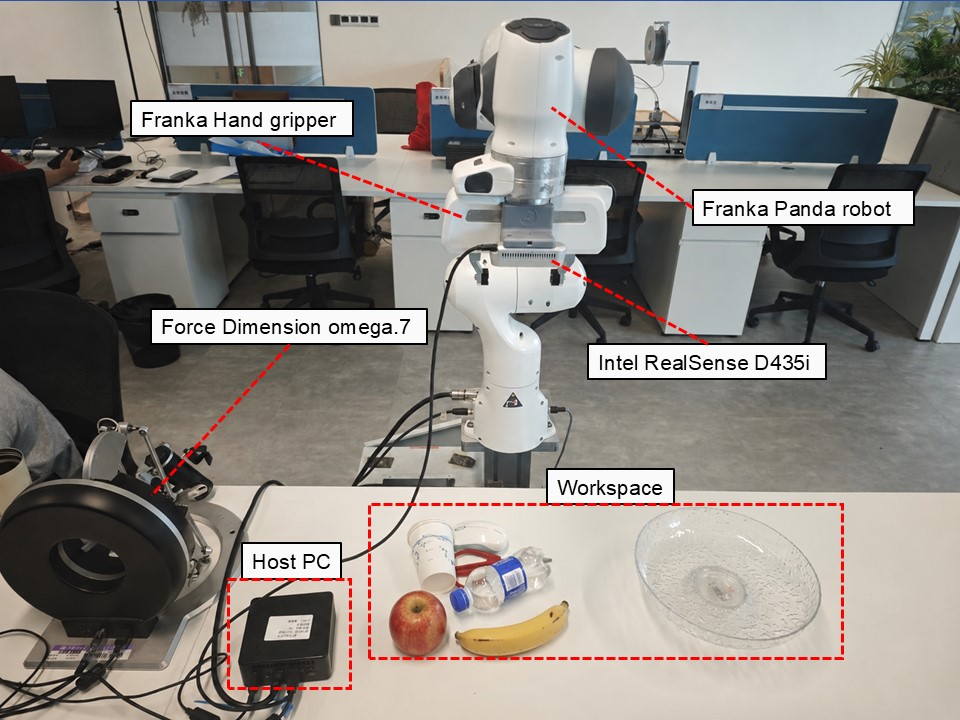
\includegraphics[width=\columnwidth]{fig1.jpg}
\caption{Experimental teleoperation platform showing the Omega.7 master device, Franka Panda robot, Intel RealSense D435i camera, host computer, and object workspace. The Franka Hand gripper is mounted at the Panda end effector.}
\label{fig:1}
\end{figure}

Figure~\ref{fig:2} illustrates the timing relationships within this multi-rate asynchronous software architecture.

RGB frames were acquired every 66.7 ms and written to a single-slot queue, preventing stale images from accumulating. YOLO11n ran in an independent process and returned class labels and confidence scores through a two-slot result queue. The nominal 200-Hz supervisory loop polled this queue every 5 ms without waiting for inference, allowing camera acquisition, perception, and operator motion to proceed in parallel. Per-image processing time was characterized separately in a controlled image test. Table~\ref{tab:1} summarizes the update timing, triggers, and data flow of the system modules.

\begin{table*}[!t]
\centering
\caption{Runtime characteristics and data flow of the multi-rate mechatronic system.}
\label{tab:1}
\small
\setlength{\tabcolsep}{6pt}
\renewcommand{\arraystretch}{1.16}
\begin{tabularx}{\textwidth}{@{}p{0.20\textwidth}p{0.24\textwidth}Y@{}}
\toprule
Module & Timing or trigger & Data flow \\
\midrule
Master input & 200 Hz & Omega.7 translational position and buttons $\rightarrow$ master-state update. \\
Slave control & 200 Hz & Desired pose and impedance parameters $\rightarrow$ Panda command. \\
Image acquisition & 15 fps (66.7 ms/frame) & D435i color stream $\rightarrow$ $424\times240$ color image. \\
YOLO11n inference & Asynchronous; controlled-test performance characterized separately & Latest available image $\rightarrow$ class and confidence. \\
Strategy scheduling & First threshold-qualified detection & Class and confidence $\rightarrow$ target $\Theta(c)$. \\
Haptic rendering & 200 Hz & Force-related state $\rightarrow$ Omega.7 force command. \\
Gripper command & Button event & Gripper input and command parameters $\rightarrow$ Franka Hand command. \\
\bottomrule
\end{tabularx}
\par\smallskip
\footnotesize\textit{Note:} YOLO11n inference is executed in an independent process and does not block the supervisory loop.
\end{table*}

\begin{figure*}[!t]
\centering
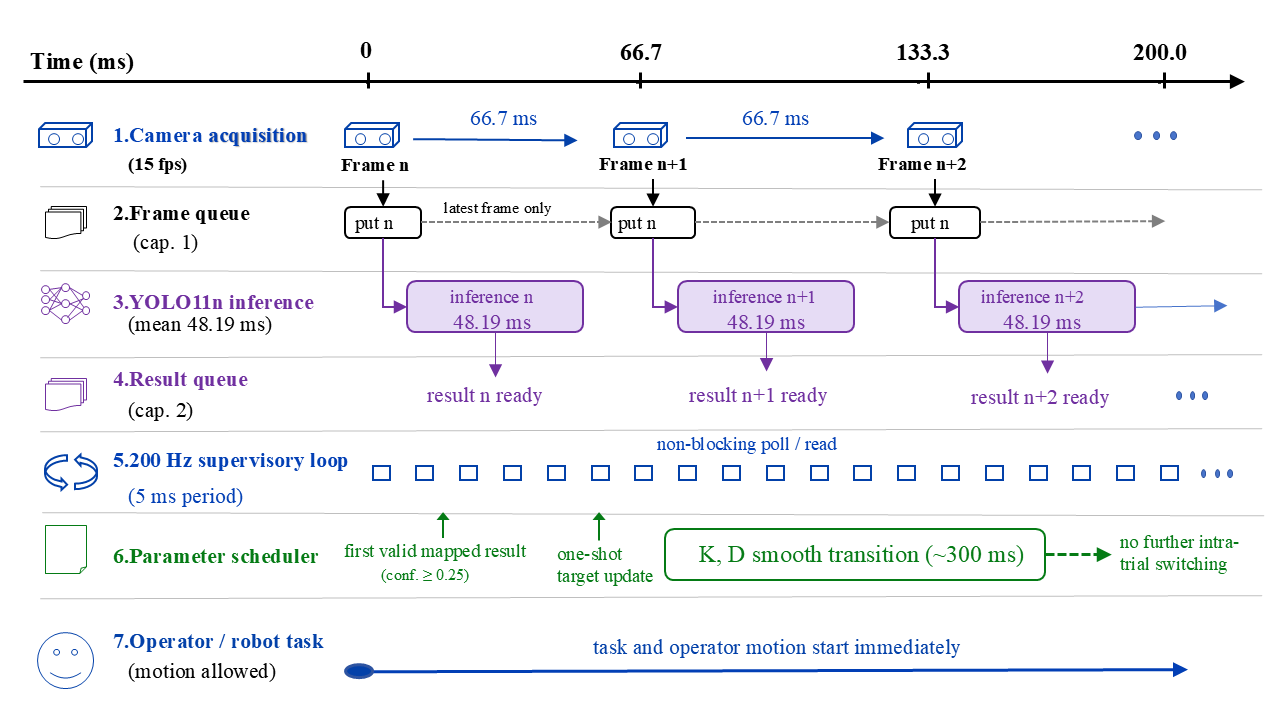
\includegraphics[width=\textwidth]{fig2.png}
\caption{Schematic, not-to-scale timing of the asynchronous perception--control implementation. Frames and results are exchanged through bounded queues while the nominal 200-Hz supervisory loop polls without blocking. The first valid mapped result ($\geq 0.25$ confidence) initiates one locked update; impedance parameters transition over approximately 300 ms. This schematic shows nominal timing, not measured end-to-end latency.}
\label{fig:2}
\end{figure*}
\subsection{Teleoperation and Mechatronic Control Channels}
\subsubsection{Master--slave motion mapping}
Only translational motion of the Omega.7 was mapped to the Panda. The master-device position increment and desired slave position were updated as

\begin{equation}
\label{eq:master-position-increment}
\Delta\mathbf{p}_m(k)=\mathbf{p}_m(k)-\mathbf{p}_m(k-1),
\end{equation}

\begin{equation}
\label{eq:desired-slave-position}
\mathbf{p}_d(k)=\mathbf{p}_d(k-1)+S\mathbf{C}\Delta\mathbf{p}_m(k),
\end{equation}

where the position-scaling factor was $S=3.0$ and $\mathbf{C}=\mathrm{diag}(-1,-1,1)$. The desired end-effector orientation $\mathbf{R}_d$ was fixed at its prescribed value throughout each trial; active rotational input from the operator was not mapped.

\subsubsection{Slave-side Cartesian impedance}
At a conceptual level, Cartesian impedance control acted on the six-dimensional pose error,

\begin{equation}
\label{eq:cartesian-impedance}
\mathbf{w}_c=\mathbf{K}(c)\mathbf{e}+\mathbf{D}(c)\dot{\mathbf{e}},
\end{equation}

\begin{equation}
\label{eq:stiffness-matrix}
\mathbf{K}(c)=\mathrm{diag}(K_t,K_t,K_t,K_r,K_r,K_r),
\end{equation}

where $\mathbf{e}$ contains translational error relative to $\mathbf{p}_d$ and rotational error relative to the fixed $\mathbf{R}_d$. Thus, $K_r$ changes resistance to rotational disturbances and the ability to hold the prescribed orientation; it does not scale operator-commanded rotation. Here $\mathbf{D}$ denotes the controller's effective damping action rather than an independently identified physical Cartesian damping matrix.

The slave-controller API internally generated its normalized damping action from the active diagonal stiffness matrix and a scalar API parameter denoted by $\zeta$. In the implementation convention,

\begin{equation}
\label{eq:damping-matrix}
\mathbf{D}_{\mathrm{API}}(c)=2\zeta(c)\sqrt{\mathbf{K}(c)},
\end{equation}

where the square root is applied elementwise to the diagonal entries. $\mathbf{D}_{\mathrm{API}}$ denotes the API's normalized internal construction and is not reported as a physical damping matrix in SI units. Accordingly, $\zeta$ is treated only as the dimensionless damping-scaling parameter exposed by the controller API and is not interpreted as a Cartesian critical-damping ratio, because no effective Cartesian mass or inertia matrix was identified.

\subsubsection{Master-side haptic rendering}
For haptic rendering, the Franka internal state estimator provided the slave-side external-force estimate $\mathbf{F}_{\mathrm{ext}}$ in newtons. The baseline master-side force command along direction $i$ was

\begin{equation}
\label{eq:baseline-haptic-command}
u_{h,i}^{\mathrm{base}}=
\operatorname{sgn}\!\left(K_fF_{\mathrm{ext},i}\right)
\max\!\left(\left|K_fF_{\mathrm{ext},i}\right|-d,0\right),
\quad i\in\{x,y,z\},
\end{equation}

where $K_f$ is a dimensionless force-scaling factor and $d$ is a per-axis dead-zone threshold in newtons.

A separate positive-$z$ cue was generated solely from the Omega.7 gripper angle $\theta_{\Omega}$:

\begin{equation}
\label{eq:gripper-cue-activation}
\alpha_g=\operatorname{clip}\!\left(
\frac{\theta_{\max}-\theta_{\Omega}}
{\theta_{\max}-\theta_{\min}},0,1\right),
\end{equation}

\begin{equation}
\label{eq:gripper-cue-command}
u_g=\min\!\left(\alpha_gG_{\mathrm{cue}}F_{\mathrm{cue,max}},F_{\mathrm{cue,max}}\right),
\qquad
u_{h,z}=u_{h,z}^{\mathrm{base}}+u_g.
\end{equation}

With $G_{\mathrm{cue}}=0.3$ and $F_{\mathrm{cue,max}}=1.0$ N, the cue was $u_g=0.3\alpha_g$ N and therefore remained within $[0,0.3]$ N. It was updated during every nominal 200-Hz supervisory cycle, with a more open Omega.7 gripper producing a larger cue. This cue was derived solely from the Omega.7 gripper aperture and did not encode slave-gripper aperture or measured grasp force.

\subsubsection{Gripper-execution channel}
For gripper execution, $v_g$ was passed as the \texttt{speed} argument of the \texttt{grasp} API, whose remaining arguments were \texttt{width}, \texttt{force}, \texttt{epsilon\_inner}, and \texttt{epsilon\_outer}; it was also used by \texttt{move} during opening and non-grasp position adjustments. The strategy value $F_g$ specified the requested \texttt{force} argument of \texttt{grasp()} in newtons; it was not an independently measured fingertip force. The target grasp width was 0 m. In the experimental implementation, \texttt{epsilon\_inner} was 0.005 m and \texttt{epsilon\_outer} was 0.080 m (the maximum gripper aperture); these fixed tolerances defined the inner and outer width bounds used by the \texttt{grasp()} success criterion and did not vary by strategy. The fixed target width and tolerances ensured a common grasp-success criterion across strategies. After contact and successful entry into the \texttt{HOLDING} state, the grasp command was not repeatedly retransmitted; the gripper maintained the grasp internally until \texttt{stop()} and the subsequent release or opening command.

The three channels act on distinct parts of the teleoperation system: Panda impedance determines the slave-side response to pose error and disturbance, Omega.7 settings render the estimated external force to the operator, and Franka Hand settings govern grasp execution. The proposed framework coordinates them through a common strategy-level parameter bundle.

\subsection{Object-Conditioned Joint Parameter Configuration}
\subsubsection{Class-to-strategy and strategy-to-parameter mapping}
The framework uses a three-level mapping from detected object class to an operational strategy and then to a joint parameter vector,

\begin{equation}
\label{eq:strategy-vector}
\Theta(c)=\{K_t,K_r,\zeta,K_f,d,v_g,F_g\}.
\end{equation}

The strategy classes represent combined grasping risks rather than material softness alone. The mapping follows an explicit engineering chain from object characteristics and manipulation risks to desired operating behavior and parameter directions. The apple and banana were assigned to the fragility-priority strategy because lower contact impact, closing speed, and requested grasp force were preferred to limit squeezing and deformation, while their smooth surfaces still posed a risk of slip. The paper cup and bottle were assigned to the balanced strategy. Excessive force can deform a paper cup, whereas overly low settings may produce an insecure grasp; the bottle similarly requires a compromise between gentle handling and slip resistance. The mouse and scissors were assigned to the stability-priority strategy because their smooth or irregular surfaces and transfer demands---and, for the scissors, elongated geometry---placed greater emphasis on pose retention and grasp stability. These assignments were specific to the present objects, platform, and task; the associated parameter settings are listed in Table~\ref{tab:2}.

\begin{table*}[!t]
\centering
\caption{Parameter settings for the three operational strategies. $K_t$ is in N/m, $K_r$ in N\,m/rad, $d$ in N, $v_g$ in m/s, and $F_g$ is the requested \texttt{grasp()} force in N. $\zeta$ and $K_f$ are dimensionless controller/API scaling parameters.}
\label{tab:2}
\small
\setlength{\tabcolsep}{6pt}
\renewcommand{\arraystretch}{1.16}
\begin{tabularx}{\textwidth}{@{}p{0.18\textwidth}p{0.20\textwidth}YYY@{}}
\toprule
Strategy & Assigned objects & Slave impedance & Haptic interface & Gripper \\
\midrule
Fragility-priority & Apple, banana & $K_t=50$ N/m; $K_r=5$ N\,m/rad; $\zeta=0.8$ & $K_f=0.2$; $d=0.3$ N & $v_g=0.02$ m/s; $F_g=8$ N \\
Balanced & Paper cup, bottle & $K_t=150$ N/m; $K_r=10$ N\,m/rad; $\zeta=1.0$ & $K_f=0.5$; $d=0.4$ N & $v_g=0.05$ m/s; $F_g=15$ N \\
Stability-priority & Mouse, scissors & $K_t=200$ N/m; $K_r=13$ N\,m/rad; $\zeta=1.2$ & $K_f=0.7$; $d=0.5$ N & $v_g=0.10$ m/s; $F_g=20$ N \\
\bottomrule
\end{tabularx}
\end{table*}
\subsubsection{One-shot triggering, locking, and parameter transition}
At run time, the first threshold-qualified result read by the supervisory loop triggered a one-time update of the parameters enabled in the active mode, after which the strategy remained locked for the rest of the trial. Translational stiffness, rotational stiffness, and the damping-scaling parameter followed a smoothstep interpolation over approximately $T_s=0.30$ s. With $\tau=\operatorname{clip}((t-t_0)/T_s,0,1)$ and $s(\tau)=3\tau^2-2\tau^3$, each interpolated quantity $q\in\{K_t,K_r,\zeta\}$ was updated as

\begin{equation}
\label{eq:smoothstep-update}
q(t)=q_0+s(\tau)(q_\mathrm{target}-q_0).
\end{equation}

The smoothstep interpolation yields continuous trajectories for $K_t$, $K_r$, and $\zeta$, with zero update rate at the start and end of the transition. It was introduced to reduce discontinuities in the commanded impedance parameters and is not interpreted as a formal transient-stability guarantee for the complete teleoperation system.

The controller recomputed $\mathbf{D}_{\mathrm{API}}$ from the current $\mathbf{K}$ and $\zeta$ during this transition. Enabled values of $K_f$, $d$, $v_g$, and $F_g$ changed immediately at the strategy event.

The class-to-strategy mapping is manually engineered. It converts a recognized known-object class into a constrained, repeatable operating strategy spanning the three subsystems; it does not infer physical properties directly. A new object must first be assigned a stable detector label and an explicit strategy entry before it can invoke a parameter bundle.

Figure~\ref{fig:3} summarizes the class-to-strategy mapping, the one-shot configuration event, and the three parameter channels.
\begin{figure*}[!t]
\centering
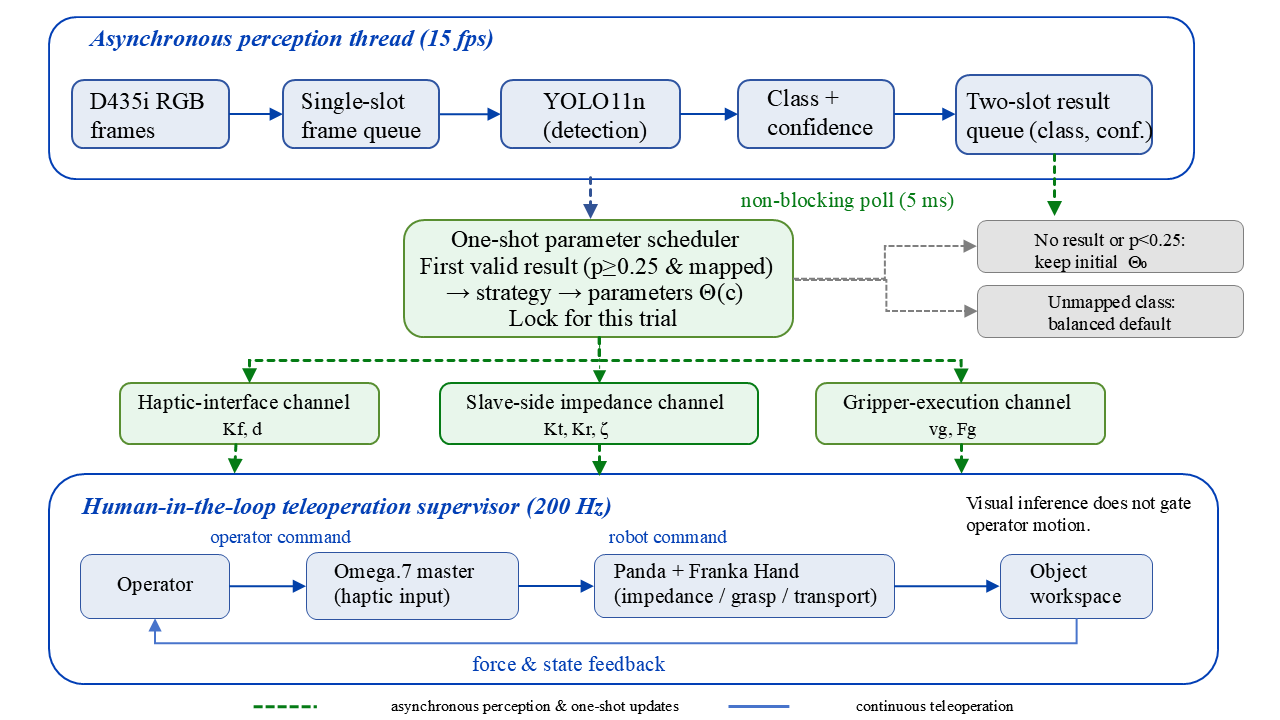
\includegraphics[width=\textwidth]{fig3.png}
\caption{Object-conditioned joint parameter-configuration architecture. D435i RGB frames are processed asynchronously by YOLO11n and returned as class--confidence results through bounded queues. The 200-Hz teleoperation supervisor polls the result queue without blocking. The first mapped result with confidence $\geq 0.25$ is converted into one strategy event $\Theta(c)$, which assigns the haptic-interface, slave-side impedance, and gripper-execution parameter groups and is locked for the trial. The diagram also shows the retained initial state for no or low-confidence results, the balanced default for an unmapped class, and the continuous operator--robot force/state-feedback loop.}
\label{fig:3}
\end{figure*}

\subsection{Parameter Design and Initial State}
The fixed baseline vector was

\begin{equation}
\label{eq:baseline-parameter-vector}
\Theta_0=(150,\ 10,\ 1.0,\ 0.5,\ 0.3,\ 0.10,\ 20),
\end{equation}

with the same element order as $\Theta(c)$. The three strategy-level parameter sets were fixed before the formal experiment and were retained as the initial state whenever no automatic update occurred.

\subsubsection{Engineering rationale for operating points}
The three engineering-selected operating points were qualitatively screened on representative objects before formal data collection. Settings associated with sustained oscillation, noticeable haptic discomfort, grasp failure, or visible damage were excluded. The final settings in Table~\ref{tab:2} were fixed before the 135 trials and should not be interpreted as optimized values or material-specific damage limits; the design rationale is reported in Supplementary Table~S4.
\subsection{Runtime Procedure}
\textbf{Algorithm 1: Object-conditioned joint-parameter scheduling}

\begin{enumerate}
\item Load the initialization specified by the active experimental mode, start the nominal 200-Hz supervisory update, and launch the visual process only in modes C--E.
\item Poll the visual-result queue without blocking while executing teleoperation, haptic rendering, and gripper control.
\item While the strategy is unlocked, retain the initialized state when no result is available or confidence is below threshold. For a threshold-qualified result, select the mapped strategy; use the balanced strategy when the detected class is not explicitly mapped.
\item Update only the parameter channels enabled by the active mode. Interpolate $K_t$, $K_r$, and $\zeta$ over approximately 300 ms; update enabled haptic-interface and gripper settings immediately.
\item Lock the selected strategy for the remainder of the trial and ignore subsequent visual results for parameter configuration.
\item Record the active parameter state, task trajectory, duration, and outcome, and reset the system after the prescribed terminal procedure.
\end{enumerate}
\subsection{Bounded Fallback and Safety Measures}
A misclassification as another known class invoked the strategy assigned to that class. A detected label without an explicit mapping invoked the balanced default strategy, whereas a missing or low-confidence detection caused no update. Every fallback outcome was confined to one of the three predefined parameter sets, although a bounded parameter set may still be inappropriate for a misclassified object.

In addition to these software fallbacks, robot collision detection, Franka Hand force settings, zero-force commands on exit, a standardized initial pose, and a manual emergency stop provided operational safeguards. The Omega.7 was operated using its standard driver and hardware configuration. The implemented mapping limited the additional master-gripper-aperture cue to 0.3 N. The baseline force-feedback command was transmitted without an additional software saturation layer, and saturation status was not logged.
